
\documentclass[11pt,twoside=false,open=any]{scrbook}

\usepackage[utf8]{inputenc}
\usepackage[ngerman]{babel}
\usepackage{skript2016}

\usepackage{siunitx}
\usepackage{wrapfig}
\usepackage{nicefrac}
\tcbuselibrary{breakable}
\usepackage{circuitikz}
\usepackage{qrcode}
\usepackage{amsmath}

\begin{document}
\title{Praktikum Sekunda}

%\author{Matthias Heimberg}
\publishers{Online verfügbar unter \href{https://goo.gl/6QeQWj}{goo.gl/6QeQWj}}
\date{Sekunda, 2017}

\begingroup
 \makeatletter
 \@titlepagetrue
 \maketitle
\endgroup
\newpage

\newcounter{aufgaben}
\tableofcontents
\newpage
\chapter{Die Grundgrössen der Elektrizität} %https://drive.google.com/file/d/0B4nWIuz6_aEMdEs5S3FwMVlJems/view
\section{Der Aufbau eines Atoms}
Alle Körper sind aus Atomen aufgebaut. Ein Atom besteht aus einem positiv geladenen Atomkern, der von einer negativ geladenen Atomhülle umgeben ist. In der Atomhülle befinden sich negativ geladene Elektronen. Im Atomkern befinden sich positiv geladene Protonen. Ein Elektron besitzt die kleinste negative Ladung: $-1e$. Ein Proton besitzt die kleinste negative Ladung: $+1e$. Ein Atom ist nach aussen elektrisch neutral (elektrisch ungeladen), wenn sich genauso viele Elektronen in der Atomhülle wie Protonen im Kern befinden.

\begin{figure}[h]
\centering
\begin{tikzpicture}[scale=0.9]
    \draw[fill=gray!30] (0,0) node[] {$+$} circle (2mm);
    \draw[] (0,0) circle (2cm);
    \draw[fill=white] (2,0) node[] {$-$} circle (1.5mm);
\end{tikzpicture}
\caption{Wasserstoffatom im Schalenmodell}
\label{fig:wasserstoffatom}
\end{figure}

\section{Elektrisch geladene Körper}
Ein Körper ist elektrisch geladen, wenn sich die Anzahl der positiven Ladungen aller Atomkerne von der Anzahl aller Elektronen unterscheidet. Ein elektrisch negativ geladener Körper hat Elektronenüberschuss, ein elektrisch positiv geladener hat Elektronenmangel.

\section{Elektrische Ladung}
Die physikalische Grösse elektrische Ladung beschreibt, wie stark ein Körper positiv bzw. negativ geladen ist, bzw. wie gross der Elektronenüberschuss oder der Elektronenmangel eines Körpers ist. Wir messen elektrische Ladung in der Einheit Coulomb (\si{\coulomb}) und benutzen dafür das Formelzeichen $Q$:
\[ \left[ Q \right] = \si{\coulomb} \]


\section{Elektrischer Strom in Metallen}
Elektrischer Strom ist bewegte Ladung. Im Metall können sich einige Elektronen frei bewegen. Ihre Bewegung ist ungerichtet. Wird ein metallischer Leiter mit einer Spannungsquelle verbunden, so bewegen sich die Elektronen in eine bestimmte Richtung. Am Minuspol der Spannungsquelle herrscht Elektronenüberschuss, am Pluspol Elektronenmangel. 

\section{Die elektrische Stromstärke}
\begin{center}
   \setlength{\fboxrule}{2pt}
   \fcolorbox{black}{gray!10}{
\begin{minipage}{\textwidth}
\paragraph{Definition}
Die elektrische Stromstärke ist definiert als die Rate, mit der die Ladung fliesst.  Die Definition der Stromstärke $I$ lässt sich als Gleichung schreiben:
\[ I = \frac{\Delta Q}{\Delta t} \]
wobei $\Delta Q$ die in der Zeit $\Delta t$ durch eine gegebene Fläche fliessende Ladung bezeichnet.
\end{minipage}
}
\end{center}

Eine grosse Stromstärke, wie sie zum Beispiel gebraucht wird um einen Automotor zu starten, bewegt eine grosse Ladungsmenge in einer kurzen Zeit. Eine kleine Stromstärke, wie sie in ihren Taschenrechner fliesst, bewegt eine kleine Menge Ladung über eine lange Zeitdauer.

\begin{figure}[h]
\centering
\begin{tikzpicture}[scale=0.6]
    \def\ladungq#1{
    \begin{scope}[shift={#1}]
    \draw[-latex] (0,0) -- (4,0);
    \draw[outer color=blue!70, inner color=white] (0,0) circle (0.3) node[] {$q$};
    \end{scope}
    }



    \fill[top color=gray, bottom color=white] (0,4) to [out=180,in=90] (-0.7,3) to [out=-90,in=180] (0,1.75) -- (2,1.75) -- (2,4);
    
    \fill[top color=white, bottom color=gray] (10,0) to [out=0,in=-90] (10.7,1) to [out=90,in=0] (10,2.25) -- (8,2.25) -- (8,0);
    
    \draw[] (0,4) to [out=180,in=90] (-0.7,3) to [out=-90,in=180] (0,1.7);
    
    \draw[] (10,0) to [out=0,in=-90] (10.7,1) to [out=90,in=0] (10,2.25);
    
    \draw[top color=gray!70, bottom color=gray!70, middle color=white] (0,0) to [out=180,in=-90] (-0.7,1) to [out=90,in=180] (0,2) to [out=0,in=-90] (0.7,3) to [in=0,out=90] (0,4) -- (10,4) to [out=0,in=90] (10.7,3) to [out=-90,in=0] (10,2) to [out=180,in=90] (9.3,1) to [out=-90,in=180] (10,0) --cycle;
    
    \draw[gray,thin] (5,2) ellipse (0.75 and 2);
    \draw[latex-] plot [smooth, tension=0.5] coordinates {(5,3.7) (5.6,4.7) (6.2,4.2) (6.7,4.8)} node[above] {$A$};
    \ladungq{(3.5,3.5)};
    \ladungq{(1.6,2.6)};
    \ladungq{(2.6,1.5)};
    \ladungq{(3.1,0.6)};
    
\end{tikzpicture}
    
\caption{Die elektrische Stromstärke $I$ ist definiert als die Ladungsmenge pro Sekunde, die durch eine gegebene Fläche fliesst.}
\label{fig:feldimleiter}
\end{figure}

%\begin{center}
\begin{tcolorbox}[colback=white, title=Beispiel: Berechnung von Stromstärken]
\begin{enumerate}
    \item Wie gross ist die Stromstärke einer Autobatterie, wenn zum  Starten des Motors eine Ladung von \SI{720}{C} in \SI{4.00}{s} fliesst?
    
    \item Wie lange dauert es, bis eine Ladung von \SI{1.00}{\coulomb} durch einen Taschenrechner geflossen ist, wenn die Stromstärke \SI{0.300}{\milli \ampere} beträgt?
    \end{enumerate}
\paragraph{Strategie}\mbox{}\\
    Wir können die Definition der Stromstärke aus der Gleichung $I=\nicefrac{\Delta Q}{\Delta t}$ benutzen, um die Stromstärke für Teil a. zu berechnen, da die Ladung und die Zeit gegeben sind.
    Für Aufgabe b. formen wir die Gleichung um und benutzen die gegebene Ladung und Stromstärke um die Zeit zu berechnen. 
\paragraph{Lösung für a.}\mbox{}\\
    Einsetzen der Werte für Ladung und Zeit ergibt:
    \[ I = \frac{\Delta Q}{\Delta t} = \frac{\SI{720}{C}}{\SI{4.00}{s}} = \SI{180}{\coulomb \per \second} = \SI{180}{A} \]
\paragraph{Diskussion zu a.}\mbox{}\\
    Der grosse Wert für Stromstärke illustriert die Tatsache, dass eine grosse Ladung in kurzer Zeit bewegt wird. Die Stromstärken die beim Starten eines Motors fliessen müssen gross sein, da zum Starten des Motors relativ starke Reibungskräfte überwunden werden müssen.
\paragraph{Lösung für b.}\mbox{}\\
    Auflösen der Gleichung nach der Zeit ergibt:
    \[ \Delta t = \frac{\Delta Q}{I} = \frac{\SI{1.00}{C}}{\SI{0.300E-3}{\coulomb \per \second}} = \SI{3.33E3}{s} \]
\paragraph{Diskussion zu b.}\mbox{}\\
    Es dauert etwas weniger als eine Stunde. Die geringe Stromstärke für einen Taschenrechner benötigt viel länger um eine kleinere Ladung zu bewegen als die Stromstärke im Motor. Weshalb können wir aber den Taschenrechner gleich nach dem Einschalten bereits benutzen? Ein Taschenrechner besitzt eben keine beweglichen Teile und benötigt nur sehr wenig Energie um zu funktionieren.
\end{tcolorbox}
%\end{center}

\begin{figure}[h]
\centering
\begin{tikzpicture}[scale=0.1]
    %Netzgerät
    \draw[fill=gray!30,rounded corners=2] (0,-0.2) rectangle (48,20);
    \draw[black!80,fill=black!80,rounded corners=2] (2,2) rectangle (4,5.9);
    \draw[white,thick] (3,3) circle (0.4);
    \draw[white,thick] (3,4.4) -- (3,5.2);
    \draw[fill=gray!10,rounded corners=1.5] (4,10) rectangle (15,15);
    \draw[fill=gray!10,rounded corners=1.5] (4+15,10) rectangle (15+15,15);
    \draw[fill=gray!60,gray!60] (9.5,4) circle (1.5);
    \draw[fill=gray!60,gray!60] (9.5+7.5,4) circle (1.5);
    \draw[fill=gray!60,gray!60] (9.5+15,4) circle (1.5);
    \draw[fill=red,red] (31,6) circle (0.9); %outputA+
    \draw[fill=red,red] (31+7.5,6) circle (0.9);
    \draw[fill=yellow,yellow] (34.75,4) circle (0.9);
    \draw[fill=blue,blue] (31,2) circle (0.9); %outputA-
    \draw[fill=blue,blue] (31+7.5,2) circle (0.9);
    \draw[fill=gray!60,gray!60] (43,2.5) circle (0.8);
    
    \draw[thick] (31,6) to [out=280, in=180] (60,-4.5);
    \draw[thick] (60,-4.5) to [out=0, in=270] (75,10);
    \draw[thick] (31,2) to [out=300, in=180] (60,-6);
    \draw[thick] (60,-6) to [out=0, in=270] (77,10);
    
    \draw[stealth-] (53,-3) --node[above] {$I$} (56,-3);
    \draw[-stealth] (53,-8) --node[below] {$I$} (56,-8);
    
    \draw[fill=black,rounded corners=1] (73,10) rectangle (79,13);
    \draw[fill=yellow] (76,14.3) circle (1.5);
    
    \draw[] (100,5) -- (100,-5) -- (120+10,-5) -- (120+10, 4);
    \draw[] (120+10,7) circle (3);
    \begin{scope}
        \clip (120+10,7) circle (3);
        \draw[] (115+10,2) -- ( 125+10,12);
        \draw[] (125+10,2) -- ( 115+10,12);
    \end{scope}
    \draw[] (120+10,10) -- ( 120+10,19) -- (100,19) -- (100,9);
    \draw[] (100-5,9) -- (100+5,9);
    \draw[] (100-3,5) -- (100+3,5);
    \node at (100-2,3) {$-$};
    \node at (100-2,11) {$+$};
    \draw[-stealth] (112,-2) --node[above] {$I$} (120,-2); 
    \draw[stealth-] (112,16) --node[below] {$I$} (120,16); 
\end{tikzpicture}
    
\caption{Ein einfacher elektrischer Stromkreis. Der Strom fliesst durch die Kabel von der Spannungsquelle zum Lämpchen (die physikalische Stromrichtung läuft von $-$ zu $+$. Im Schaltbild (rechts) werden für die Spannungsquelle und das Lämpchen entsprechende Symbole verwendet.}
\label{fig:elektroskop1}


\end{figure}

\newpage
Verantwortlich für den Fluss der Ladungen ist ein elektrisches Feld im Leiter. Die Bewegung der Ladungen benötigt Energie, diese wird durch das elektrische Feld bereitgestellt.

\begin{figure}[h]
\centering
\begin{tikzpicture}[scale=0.6]
    \def\ladungq#1{
    \begin{scope}[shift={#1}]
    \draw[-latex] (0,0) -- (4,0);
    \draw[outer color=blue!70, inner color=white] (0,0) circle (0.3) node[] {$q$};
    \end{scope}
    }



    \fill[top color=gray, bottom color=white] (0,4) to [out=180,in=90] (-0.7,3) to [out=-90,in=180] (0,1.75) -- (2,1.75) -- (2,4);
    
    \fill[top color=white, bottom color=gray] (10,0) to [out=0,in=-90] (10.7,1) to [out=90,in=0] (10,2.25) -- (8,2.25) -- (8,0);
    
    \draw[] (0,4) to [out=180,in=90] (-0.7,3) to [out=-90,in=180] (0,1.7);
    
    \draw[] (10,0) to [out=0,in=-90] (10.7,1) to [out=90,in=0] (10,2.25);
    
    \draw[top color=gray!70, bottom color=gray!70, middle color=white] (0,0) to [out=180,in=-90] (-0.7,1) to [out=90,in=180] (0,2) to [out=0,in=-90] (0.7,3) to [in=0,out=90] (0,4) -- (10,4) to [out=0,in=90] (10.7,3) to [out=-90,in=0] (10,2) to [out=180,in=90] (9.3,1) to [out=-90,in=180] (10,0) --cycle;
    
    \draw[gray,thin] (5,2) ellipse (0.75 and 2);
    \draw[latex-] plot [smooth, tension=0.5] coordinates {(5,3.7) (5.6,4.7) (6.2,4.2) (6.7,4.8)} node[above] {$A$};
    \ladungq{(3.5,3.5)};
    \ladungq{(1.6,2.6)};
    \ladungq{(2.6,1.5)};
    \ladungq{(3.1,0.6)};
    
    \draw[very thick,stealth-] (4,-0.5) --node[below] {E} (6,-0.5);
    \draw[very thick,-stealth] (2,4.5) --node[above] {I} (4,4.5);
\end{tikzpicture}
    
\caption{Die freien Elektronen im Leiter werden durch das elektrische Feld $E$ bewegt, so entsteht der Stromfluss $I$. Beachten Sie die Richtung von $E$ und $I$!}
\label{fig:elektroskop1}
\end{figure}

\begin{tcolorbox}[breakable,colback=white, title=Beispiel: Anzahl Elektronen die sich durch einen Taschenrechner bewegen]
Wie viele Elektronen bewegen sich pro Sekunde durch einen Taschenrechner, wenn ein Strom von \SI{0.300}{\milli \ampere} fliesst?
\paragraph{Strategie}\mbox{}\\
    Da jedes Elektron eine Ladung von \SI{-1.60E-19}{\coulomb} besitzt, können wir die Stromstärke von Coulomb pro Sekunde in Elektronen pro Sekunde umrechnen.
\paragraph{Lösung}\mbox{}\\
    Wir sterten mit der Definition der Stromstärke:
    \[ I_{Elektronen} = \frac{\Delta Q_{Elektronen}}{\Delta t} = \frac{\SI{-0.300E-3}{C}}{\si{s}}  \]
    Wir teilen dies nun durch die Ladung eines Elektrons:
    \[ \frac{\si{e}}{\si{s}} = \frac{\SI{-0.300E-3}{\coulomb}}{\si{s}} \cdot \frac{1}{\SI{-1.60E-19}{\coulomb}}  = \SI{1.88E15}{e \per \second}\]
\paragraph{Diskussion}\mbox{}\\
    Es bewegen sich so viele geladene Teilchen, auch in kleinen Strömen, dass individuelle Ladungen nicht bemerkt werden, so wie man in einem Wasserfluss auch die einzelnen Wassermoleküle nicht bemerkt. Die Ladungen bewegen sich übrigens nicht alle in der gleichen Richtung, im Leiter kollidieren sie mit den Atomen und anderen Elektronen und bewegen sich so sehr chaotisch aber in der Tendenz vorwärts.

\end{tcolorbox}

\section{Die elektrische Spannung}
Elektrischer Strom fliesst nicht von selbst, sondern benötigt eine elektrische Spannung als Ursache. Elektrische Spannung wiederum ist das Ergebnis einer Ladungstrennung, beispielsweise einer Erhöhung der Konzentration an Elektronen an einer Stelle gegenüber einer anderen Stelle.
\begin{center}
   \setlength{\fboxrule}{2pt}
   \fcolorbox{black}{gray!10}{
\begin{minipage}{\textwidth}
\paragraph{Definition}
Die elektrische Spannung $U$ zwischen 2 Punkten ist gleich der Menge an Arbeit $\Delta W$, die pro Ladung $Q$ zwischen diesen 2 Punkten verrichtet wird:
\[ U = \frac{\Delta W}{Q} \]
Die Einheit der Spannung ist das Volt:
\[ \left[ U \right] = \SI{1}{\joule \per \coulomb} = \SI{1}{\volt} \]
\end{minipage}
}
\end{center}
Die wichtigsten Punkte zur Spannung:
\begin{itemize}
    \item Die Spannung zwischen den beiden Polen einer Spannungsquelle ist anschaulich
darauf zurückzuführen, dass diese Pole unterschiedliche elektrische Ladungen 
tragen. In vielen Fällen, z.B. bei einer Batterie, herrscht am einen Pol ein Elektronenüber-
schuss (negativer Pol) und am anderen ein Elektronenmangel (positiver Pol).
    \item Muss Arbeit resp. Energie aufgewendet werden, um eine elektrische Ladung von einem
Ort $A$ zu einem Ort $B$ zu bewegen, so herrscht zwischen diesen beiden Orten eine elektrische
Spannung. Z.B. braucht es Energie, um die Pole einer Batterie aufrecht zu erhalten
resp. aufzubauen, um also Elektronen vom positiven zum negativen Pol zu bewegen und
somit die Ladungstrennung zu bewirken. ``Energielieferant'' ist der chemische Prozess im
Batterieinnern.
\item Umgekehrt wird die Energiemenge $\Delta W$ freigesetzt, wenn sich die Ladung $Q$ von $B$ nach
$A$ bewegt: $\Delta W = U \cdot Q$. Auf diese Weise erklären wir die Freisetzung von Energie beim Fliessen eines elektrischen
Stromes: Die Ladungsträger (meistens Elektronen) bewegen sich von dem fü sie
energetisch höher liegenden zum energetisch tiefer liegenden Pol der Spannungsquelle.
\end{itemize}

\begin{tcolorbox}[breakable,colback=white, title=Beispiel: Berechnung einer Energiemenge]
Eine Motorradbatterie besitzt eine Spannung von \SI{12.0}{\volt}. Die Motorradbatterie kann \SI{5000}{\coulomb} Ladung bewegen, eine \SI{12.0}{\volt} Autobatterie kann eine Ladung von \SI{60000}{\coulomb} bewegen. Wie viel Energie kann jede Batterie liefern?
\paragraph{Strategie}\mbox{}\\
    Spricht man von einer \SI{12.0}{\volt} Batterie, so meint man, dass ihre Pole eine eine Potenzialdifferenz von \SI{12.0}{\volt} aufweisen. Wenn eine solche BAtterie Ladung bewegt, so bewegt sie die Ladung durch eine Potenzialdifferenz von \SI{12.0}{\volt} und die Ladung erfährt eine Änderung der potenziellen Energie um $\Delta W_{pot} = Q \Delta U$. Um also die Energiemenge zu bestimmen, multiplizieren wir die bewegte Ladung mit der Potenzialdifferenz.
\paragraph{Lösung}\mbox{}\\
    Für die Motorradbatterie gilt $Q=\SI{5000}{\coulomb}$ und $\Delta U = \SI{12.0}{\volt}$. Die totale Energie die diese Batterie liefern kann ist:
    \[ \Delta W_{pot} = \SI{5000}{\coulomb} \cdot \SI{12.0}{\volt} = \SI{6.00E4}{\joule} \]
    Analog gilt für die Autobatterie $Q=\SI{60000}{\coulomb}$ und $\Delta U = \SI{12.0}{\volt}$. Die totale Energie die diese Batterie liefern kann ist:
    \[ \Delta W_{pot} = \SI{60000}{\coulomb} \cdot \SI{12.0}{\volt} = \SI{7.20E5}{\joule} \]
\paragraph{Diskussion}\mbox{}\\
   Spannung und Energie hängen zusammen, es sind aber unterschiedliche Grössen. Die Spannungen der Batterien sind identisch, aber die gelieferten Energien unterscheiden sich erheblich. Wenn eine Batterie entladen wird, wird ein Teil der Energie im Innern der Batterie selbst umgewandelt (in Wärme). So fällt die Spannung gegen Ende und die Scheinwerfer eines Autos leuchten nur noch schwach wenn die Batterie fast leer ist.

\end{tcolorbox}

\begin{tcolorbox}[breakable,colback=gray!20, title=Auftrag 1: Die Energiemenge im Handy-Akku]
Vorbereitung:
\begin{itemize}
    \item Suchen Sie für Ihre Gruppe einen Gruppennamen aus dem Themenkreis der Elektrizitätslehre aus. Wählen Sie dazu zum Beispiel einen Namen eines Physikers, der sich mit der Elektrizität befasst hat. Alle Gruppen haben einen eigenen Namen!
    \item Suchen Sie unter dem Link \href{https://de.wikipedia.org/wiki/Lithium-Ionen-Akkumulator}{de.wikipedia.org/wiki/Lithium-Ionen-Akkumulator} nach der heute maximal möglichen Energiedichte eines Lithium-Ionen-Akkus (der typischerweise in einem Handy verbauten Akku) und wandeln Sie diese Energiedichte in \si{\joule \per \centi \metre \cubed} um.
    \item Gehen Sie auf folgende Seite: \href{https://goo.gl/T6AzG3}{goo.gl/T6AzG3} und beantworten sie als Gruppe sämtliche Fragen. 
    
    \end{itemize}
Suchen Sie im Internet nach den notwendigen Angaben um die in ihrem Handy-Akku gespeicherte Energiemenge zu bestimmen (alle Gruppenmitglieder)! Versuchen Sie danach abzuschätzen, welche maximale Energiemenge theoretisch für ihr Handy-Akku möglich wäre (mit Hilfe der gefundenen Energiedichte und dem gegebenen Volumen, dieses muss evtl. abgeschätzt werden oder direkt gemessen, wenn das Handy geöffnet werden kann). Geben Sie als Gruppe bis Ende der zweiten Lektion ein Dokument ab, das die folgenden Punkte erfüllt:
\begin{itemize}
    \item Enthält die Namen aller Gruppenmitglieder
    \item Enthält den Handy Typ und alle für die Rechnung relevanten Daten für die Handys aller Gruppenmitglieder
    \item Enthält sämtliche Quellen für alle Angaben
    \item Enthält den Rechnungsweg und das Ergebnis für die in allen Akkus gespeicherte Energiemenge
    \item Enthält eine Angabe darüber, welche Energie heute maximal in dem jeweiligen Handy Akku gepseichert werden könnte (wie lange könnten Sie damit das Handy durchschnittlich benutzen?)
    \item Gespeichert als PDF Dokument im Sharepoint unter dem Namen ``Gruppenname-1.pdf'' (z.Bsp. Faraday-1.pdf) unter E-Learning - Physik - Abgabe
\end{itemize}


\end{tcolorbox}

%\end{document} %ERSETZEN

\chapter{Das Multimeter}
Wir benötigen im Praktikum für sämtliche Messungen am Stromkreis ein und dasselbe Gerät, das Multimeter. Das Multimeter ist ein elektronisches Gerät, das für mehrere Messgrössen einsetzbar ist. Für uns wichtig sind dabei die Messung der Spannung $U$ in Volt und die Messung der Stromstärke $I$ in Ampere. Weiter kann man mit unserem Multimeter noch den elektrischen Widerstand, die Kapazität und die Frequenz messen. 

\begin{figure}[h]
\centering
\begin{tikzpicture}
\node[anchor=south west,inner sep=0] at (0,0) {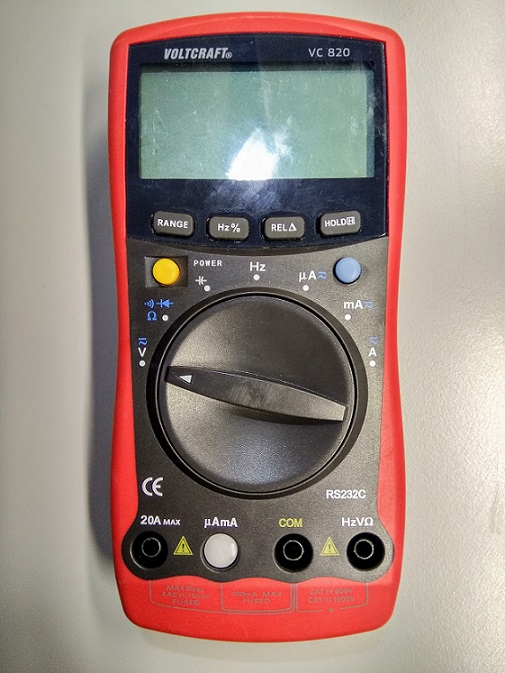
\includegraphics[scale=0.55]{Bilder/multimeter.jpg}};
\draw[thick, blue] (2.94,2.44) -- (2.94,0.7) node[below] {5};
\draw[thick, blue] (5.7,2.44) -- (5.7,0.7) node[below] {6};
\draw[thick, blue] (7.06,2.44) -- (7.06,0.7) node[below] {7};
\draw[thick, blue] (3,10.7) -- (0.75,10.7) node[left] {1};
\draw[thick, blue] (3.26,7.76) -- (0.75,7.76) node[left] {2};
\draw[thick, blue] (6.8,7.76) -- (9,7.76) node[right] {3};
\draw[thick, blue] (6.98,5.3) -- (9,5.3) node[right] {4};
\end{tikzpicture}
\caption{Das im Praktikum verwendete Multimeter: 1: LCD-Anzeige plus Anzeige der Funktionen und Masseinheiten, 2: Taster ``POWER'' für Messgerät ein / aus, 3: Taster zum Umschalten zwischen AC (Wechselstrom) und DC (Gleichstrom), 4: Drehschalter für die Einstellung der Messfunktionen, 5: 20A - (+) -Eingangsbuche  (= Plusanschluss), 6: COM (–) – Eingangsbuchse (COM – bzw. Minusanschluss), 7: Hz/V/Ohm – (+) – Eingangsbuchse (= Plusanschluss). Weitere Informationen finden Sie in der \href{https://drive.google.com/file/d/0B4nWIuz6_aEMR05PdVJFMjlaQWc/view?usp=sharing}{Bedienungsanleitung (Link)}}
\label{fig:bumerang}
\end{figure}

\section{Messung der Stromstärke mit dem Multimeter}
Das Strommessgerät wird immer in Reihe zum Verbraucher angeschlossen. Dazu muss die Leitung des Stromkreises aufgetrennt werden, um das Messgerät in den Stromkreis einfügen zu können. Während der Messung der Stromstärke muss der zu messende Strom durch das Messgerät fliessen. Zunächst wird am Drehschalter die entsprechende Einstellung (\si{\ampere}) gewählt (man kann das Multimeter jetzt als Amperemeter bezeichnen). Danach werden die Kabel in die beiden benötigten Buchsen gesteckt (20A Eingangsbuchse und COM-Anschluss). Nun muss der Stromkreis an der zu messenden Stelle geöffnet werden, und das Mulitmeter muss in Reihe zu den stromführenden Bauteilen geschaltet werden. Die Abbildung \ref{fig:stromstärke} zeigt eine Messung der Stromstärke des durch das Lämpchen fliessenden Stromes (oder kurz die Messung des Stromes durch das Lämpchen).

\begin{figure}[h]
\centering
\includegraphics[scale=0.45]{Bilder/stromstärke.jpg}
\caption{Messung des durch das Lämpchen fliessenden Stroms mit Hilfe des Multimeters. Tipp: Gehen Sie einmal mit dem Finger den Weg des Stromes durch (eine geschlossene Linie vom Minus- zum Pluspol!}
\label{fig:stromstärke}
\end{figure}

\section{Messung der Spannung mit dem Multimeter}

\begin{figure}[h]
\centering
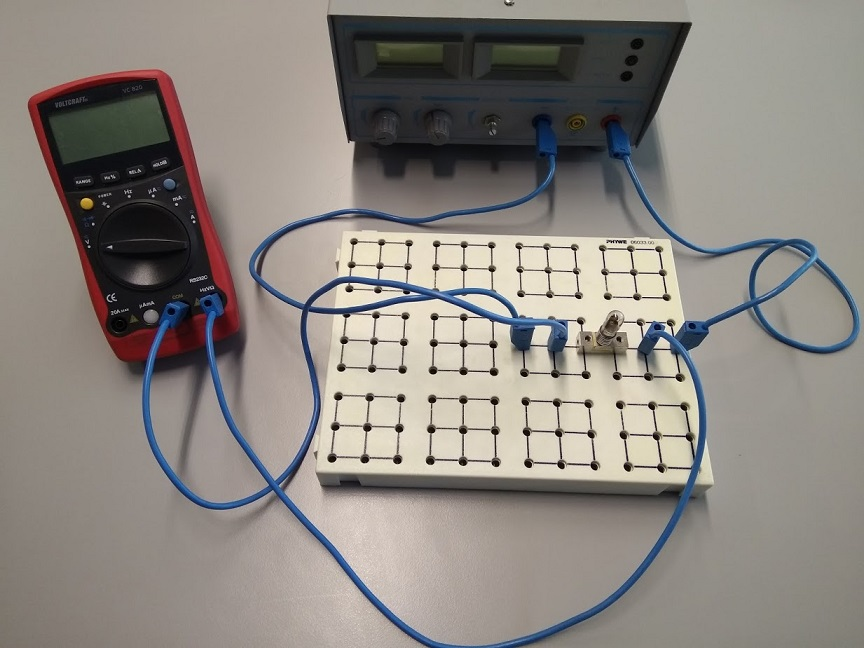
\includegraphics[scale=0.45]{Bilder/spannung.jpg}
\caption{Messung des Spannungsabfalls über einem Lämpchen mit Hilfe des Multimeters. Tipp: Gehen Sie auch hier einmal mit dem Finger den Weg des Stromes durch (eine geschlossene Linie vom Minus- zum Pluspol!}
\label{fig:spannung}
\end{figure}

Ein Spannungsmessgerät wird immer parallel zum Verbraucher, Bauelement oder zur Spannungsquelle angeschlossen. Bei der Messung an der Spannungsquelle wird der momentane Spannungswert gemessen. Am Verbraucher wird der Spannungsabfall an diesem einen Bauelement gemessen. Das ist die Teilspannung von der Gesamtspannung der Spannungsquelle. Bei der Spannungsmessung stellt das Messgerät im Idealfall einen unendlich grossen Widerstand dar, so dass kein Strom durch das Gerät fliessen kann. Zunächst wird am Drehschalter die entsprechende Einstellung (\si{\volt}) gewählt (man kann das Multimeter jetzt als Voltmeter bezeichnen). Danach werden die Kabel in die beiden benötigten Buchsen gesteckt (Hz/V/Ohm Eingangsbuchse und COM-Anschluss). Nun muss das Mulitmeter in Reihe zu den stromführenden Bauteilen geschaltet werden. Die Abbildung \ref{fig:spannung} zeigt eine Messung der Spannung (des Spannungsabfalls) über dem Lämpchen.




\begin{tcolorbox}[breakable,colback=gray!20, title=Auftrag 2: Erste Messungen mit dem Multimeter]
Um den korrekten Umgang mit dem Multimeter einzuüben, erfüllen Sie als Gruppe die folgenden Aufträge:
\begin{itemize}
    \item Öffnen Sie den Link \href{https://goo.gl/vYAZz7}{goo.gl/vYAZz7} und beantworten Sie alle Fragen!
    \item Lesen Sie nun (falls Sie dies noch  nicht gemacht haben) alles in diesem Kasten durch!
    \item Stecken Sie mit den vorgegebenen Bauteilen eine elektrische Verbindung vom Punkt $A$ zum Punkt $B$ (so dass ein Strom fliessen kann), jedes Bauteil muss \textit{sinnvoll}, d.h. als Stromleiter, verwendet werden (vgl. Abbildung \ref{fig:bauteile}). Machen Sie eine Fotografie und laden Sie die Bilddatei unter dem Namen Gruppenname-1.jpg im Sharepoint hoch.
    \item Messung 1: Stecken Sie die beiden Lämpchen hintereinander ein (in Serie) und messen Sie den durch ein Lämpchen fliessenden Strom. Am Netzgerät stellen Sie eine Spannung von (maximal) \SI{24}{Volt} ein
    \item Messung 2: Stecken Sie die beiden Lämpchen hintereinander ein (in Serie) und messen Sie die über einem Lämpchen abfallenden Spannung. Am Netzgerät stellen Sie eine Spannung von (maximal) \SI{24}{Volt} ein
\end{itemize}


Benötigtes Material für Messung 1 \& 2:
\begin{itemize}
    \item 1 Netzgerät
    \item 1 Steckbrett
    \item 2 Lämpchen (\SI{12}{V} / \SI{100}{mA})
    \item 1 Messgerät
    \item 4 Kabel (blau)
\end{itemize}
Erstellen Sie ein Dokument, das die folgenden Punkte enthält:
\begin{itemize}
    \item Gruppenname
    \item Titel: Messung der Stromstärke und der Spannung in einem einfachen Stromkreis
    \item Je eine Fotografie vom Aufbau der Messung 1 und der Messung 2 (komplett inklusive Netzgerät, wie z.Bsp. Abbildung \ref{fig:spannung})
    \item Je ein gezeichneter vollständiger Schaltplan vom Aufbau der Messung 1 und der Messung 2 mit den entsprechenden Symbolen (informieren Sie sich im Internet über die Symbole des Volt- und Amperemeters, die anderen benötigten Symbole finden Sie alle in diesem Dokument)
    \item Sämtliche Messwerte der beiden Messungen
    \item Erklären Sie anhand der gemessenen Werte die Begriffe ``Stromstärke'' und ``Spannung'' (vgl. Kapitel 1) und begründen Sie die gemessenen Werte!
\end{itemize}
Speichern Sie das Dokument bis spätestens heute in einer Woche (Montag 24:00 Uhr) als PDF unter dem Namen ``Gruppenname-2.pdf'' im Sharepoint (E-Learning  - Physik - Abgabe - ensprechender Unterordner) ab! Für den Bericht gibt es maximal 3 Punkte. Kriterien sind: Termingerechte Abgabe, Vollständigkeit, inhaltliche Richtigkeit.
\end{tcolorbox}

\begin{figure}[h]
\centering
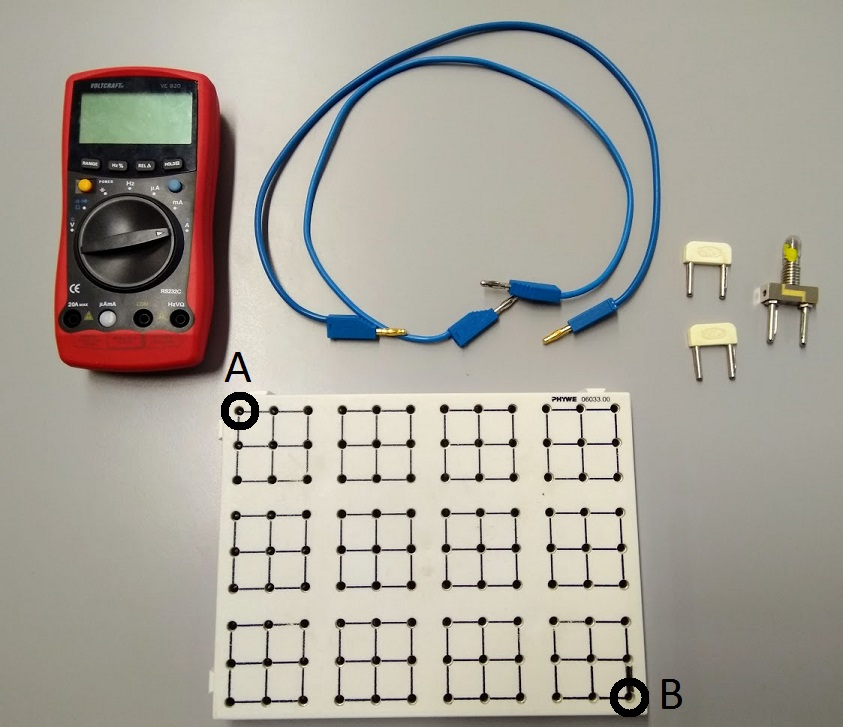
\includegraphics[scale=0.5]{Bilder/bauteile.jpg}
\caption{Die verwendeten Bauteile für Auftrag 2}
\label{fig:bauteile}
\end{figure}



%Spannung, Widerstand, Ohmsches gesetz, multiple choice fragen gruppeneinteilung messgeräte steckbrett usw


\chapter{Elektrischer Widerstand \& das ohmsche Gesetz}
Was treibt den Strom (die bewegten Elektronen) an? Es braucht jeweils ein bestimmtes Gerät, wie zum Beispiel eine Batterie, einen Generator, eine Steckdose usw. um einen Stromfluss anzutreiben. All diese Geräte stellen eine sogenannte Potenzialdifferenz her, und werden daher Spannungsquellen genannt. Wird eine Spannungsquelle an einen Leiter angeschlossen, so entsteht dadurch eine Potenzialdifferenz $U$ im Leiter, was wiederum ein elektrisches Feld in diesem Leiter erzeugt. Das elektrische Feld bringt nun die Elektronen in Bewegung.

\section{Das ohmsche Gesetz} 
Der in einem Leiter fliessende Strom (die Stromstärke) ist in den Meisten Materialien direkt proportional zur angelegten Spannung $U$. Der deutsche Physiker Georg Simon Ohm (1787-1854) war der Erste, der experimentell nachweisen konnte, dass der in einem Metalldraht fliessende Strom direkt proportional zur angelegten Spannung ist (doppelte Spannung ergibt doppelte Stromstärke):
\[ I \sim U \]
Diese wichtige Beziehung ist bekannt als das ohmsche Gesetz. Es ist ein empirisches Gesetz; also ein experimentell beobachtetes Phänomen. Der lineare Zusammenhang des ohmschen Gesetzes gilt nicht immer!

\section{Elektrischer Widerstand und einfache Stromkreise}
Wie kann der in einem Leiter fliessende Strom beeinflusst werden? Die elektrische Grösse, die den Stromfluss reguliert, ist der elektrische Widerstand $R$ (vergleichbar mit Reibung oder Luftwiderstand). Die bewegten Elektronen im Leiter kollidieren mit den Atomen und Molekülen des Materials und übertragen so Energie in die leitende Substanz und limitieren den Stromfluss. 

\begin{center}
   \setlength{\fboxrule}{2pt}
   \fcolorbox{black}{gray!10}{
\begin{minipage}{\textwidth}
\paragraph{Definition}
Der elektrische Widerstand ist invers proportional (umgekehrt proportional) zum Stromfluss:
\[ I \sim \frac{1}{R} \]
Der Stromfluss (Stromstärke) $I$ halbiert sich also, wenn der Widerstand $R$ verdoppelt wird. Kombiniert man nun die Gleichung $I \sim U$ mit $I \sim \frac{1}{R}$, so erhält man:
\[ I = \frac{U}{R} \text{ oder } U = R \cdot I \]
\end{minipage}
}
\end{center}

Die Beziehung oben nennt man auch das ohmsche Gesetz. Das ohmsche Gesetz definiert in dieser Form tatsächlich den Widerstand in bestimmten Materialien. Aber das ohmsche Gesetz ist nicht universell gültig, es gilt nur in den sogenannt ``ohmschen'' Materialien (z.Bsp. gute Leiter wie Kupfer, Aluminium). Ohmsche Materialien besitzen einen konstanten elektrischen Widerstand $R$  der unabhängig von der Spannung $U$ und der Stromstärke $I$ ist. Die Einheit für den elektrischen Widerstand ist das Ohm $\Omega$:
\[ \SI{1}{\ohm} = \SI{1}{\volt \per \ampere} \]

\begin{figure}[h]
\centering

  \begin{circuitikz}[european]
    \draw[] (0,0)
    to[battery1, l=$U_{0}$] (0,2)
    to[short] (2,2)
    to[R=$R$] (2,0)
    to[short] (0,0);
\end{circuitikz} 

\caption{Ein einfacher elektrischer Stromkreis: Die Spannungsquelle ist über einen Leiter an den Widerstand $R$ angeschlossen. }
\label{fig:parallel}
\end{figure}

\begin{tcolorbox}[breakable,colback=white, title=Beispiel: Berechnung des Widerstandes eines Autoscheinwerfers]
Wie gross ist der elektrische Widerstand einers Scheinwerfers, wenn ein Strom von \SI{2.50}{\ampere} bei einer angelegten Spannung von \SI{12.0}{\volt} fliesst?
\paragraph{Strategie}\mbox{}\\
    Das ohmsche Gesetz lässt sich nach $R$ auflösen.
\paragraph{Lösung}\mbox{}\\
    $I=\frac{U}{R}$ auflösen nach $R$, Werte einsetzen:
    \[ R = \frac{U}{I} = \frac{\SI{12.0}{\volt}}{\SI{2.50}{\ampere}}= \SI{4.80}{\ohm} \]
\paragraph{Diskussion}\mbox{}\\
   Dies ist ein relativ kleiner Widerstand, aber immer noch grösser als der Widerstand der kalten Lampe. Der Widerstand der meisten Materialien verändert sich mit der Temperatur, meistens nimmt er bei einer Erhöhung der Temperatur zu, somit fliesst beim Einschalten einer Lampe kurz ein grösserer Strom, als im laufenden Betrieb. Deshalb gehen Glühbirnen meisten sbeim einschalten kaputt.

\end{tcolorbox}

Elektrischer Widerstand kann in unterschiedlichen Materialien Werte über mehrere Grössenordnungen annehmen. Einfache Keramik-Isolatoren, wie sie zum Beispiel in Hochspannungsleitungen verwendet werden, besitzen Widerstände von \SI{1E12}{\ohm} und mehr. Eine (trockene) Person kann einen Widerstand (zwischen Hand und Fuss) von \SI{1E5}{\ohm} haben. Der elektrische Widerstand des menschlichen Herzens beträgt ungefähr \SI{1E3}{\ohm}. Ein \SI{1}{m} langes, dickes Stück Kupferdraht besitzt einen Widerstand von ca. \SI{1E-5}{\ohm} und Supraleiter besitzen überhaupt keinen elektrischen Widestand. Der elektrische Widerstand hängt von der Form und dem Material eines Objektes ab. 

Wird die Gleichung des ohmschen Gesetzes nach $U$ aufgelöst, erhalten wir:
\[ U = I \cdot R \]
Dieser Ausdruck für $U$ kann als Spannungsabfall über dem Widerstand interpretiert werden, der durch den fliessenden Strom $I$ erzeugt wird. Die Spannung kann mit dem Druck in einer Wasserleitung verglichen werden; die Spannungsquelle wirkt wie eine Wasserpumpe, die eine Drcukdifferenz und damit einen Wasserfluss herstellt. Der Widerstand ist wie ein enges Rohr, das den Druck vermindert und den Wasserfluss einschränkt. Die Energieerhaltung hat wichtige Konsequenzen im Stromkreis; Die Spannungsquelle liefert Energie und der Widerstand wandelt diese Energie in eine andere Form um. In einem einfachen Stromkreis (eine Spannungsquelle, ein Widerstand) entspricht die Spannungsdifferenz über dem Widerstand immer der Spannung der Spannungsquelle. Unter dem Link \href{https://phet.colorado.edu/sims/html/ohms-law/latest/ohms-law_de.html}{goo.gl/gmLSiv} können Sie das ohmsche Gesetz an einem einfachen elektrischen Stromkreis untersuchen.

\begin{tcolorbox}[breakable,colback=gray!20, title=Versuch 1: Kennlinie von Glühlampe und Widerstandselement]
Beantworten Sie zunächst in der Gruppe die Fragen unter \href{https://goo.gl/ByKO7H}{goo.gl/ByKO7H}, gehen Sie dann zum Versuch über: \newline
In diesem Versuch werden Sie eine sogenannte Kennlinie messen. Dazu messen Sie die Spannung $U$ und Stromstärke $I$ einer Glühlampe/eines Widerstandes. Mit den Messwerten werden Sie dann Diagramme wie das folgende erstellen:

\begin{center}
   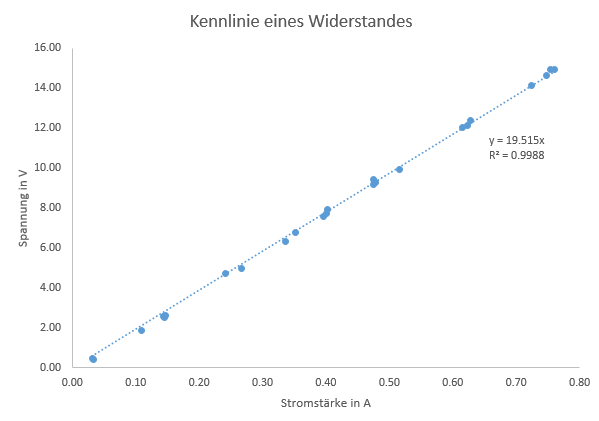
\includegraphics[width=12cm]{Bilder/Kennlinie1.png}
\end{center}



Das Diagramm erstellen Sie mit Hilfe von Microsoft Excel. Jedes Diagramm beinhaltet wie die obenstehende Vorlage eine Trendlinie und einen Diagrammtitel. Alle Achsen müssen beschriftet sein. Sie erstellen dann mit Hilfe von Microsoft Word ein Dokument, das die folgenden Punkte enthält:
\begin{itemize}
    \item Titel des Versuches (vgl. Titel dieses Kästchens)
    \item Gruppenname
    \item Ziel des Versuches 
    \item Sämtliche gemessenen Daten (beschriftete Tabelle)
    \item Je ein Diagramm zum Widerstand und zur Glühlampe (nach Vorgabe oben)
    \item Interpretation der Diagramme
    \item Quellenangaben für Abbildungen und verwendete Literatur
\end{itemize}

Für die Messung der Kennlinien benötigen Sie:
\begin{itemize}
    \item 4 blaue Kabel
    \item 2 Multimeter
    \item 1 Steckbrett
    \item 1 Widerstandselement \SI{200}{\ohm} (vgl. Farbcode-Tabelle am Ende von Kapitel 3)
    \item 1 Glühbirne \SI{12}{V} mit Fassung
    \item einige Steckverbindungen
\end{itemize}
Messen Sie Spannungen zwischen 0 bis \SI{12}{V}. Höhere Spannungen können den Widerstand oder das Lämpchen beschädigen!
\end{tcolorbox}

\begin{figure}[h]
\centering
   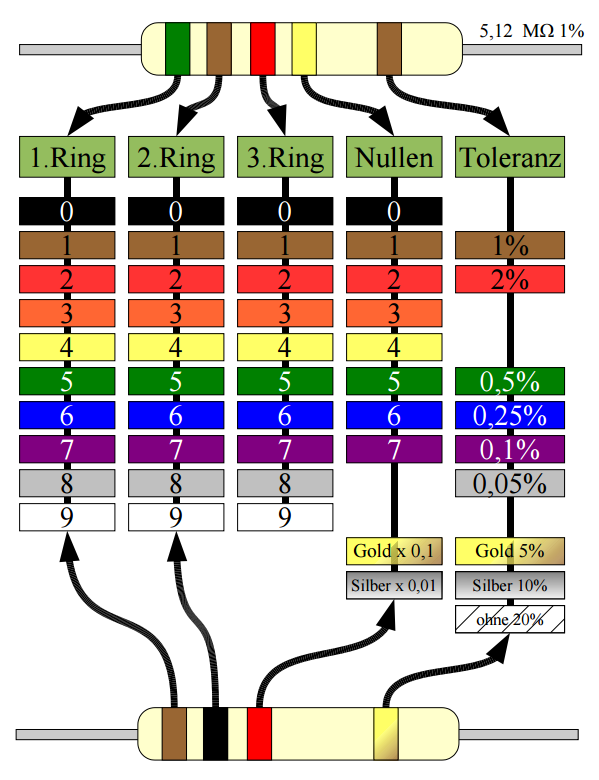
\includegraphics[width=12cm]{Bilder/Widerstand.png}
\caption{Widerstands-Farbtabelle}
\label{fig:widerstand}
\end{figure}

\end{document}

\chapter{Widerstände in Serie- und Parallelschaltung}
Elektrische Stromkreise sind allgegenwärtig. Einige sind einfach, wie zum Beispiel die Stromkreise in Taschenlampen. Andere, wie diejenigen in Supercomputer, sind extrem komplex. Wir betrachten in diesem Kapitel die einfachen, grundlegenden Arten von Stromkreisen und beschränken uns auf die Gleichspannung (DC). Einer der wichtigsten Komponenten ist das Widerstandselement (Widerstand). Ein Widerstand hat die Aufgabe den Fluss der Elektronen, also die Stromstärke im Stromkreis zu beschränken. Die einfachsten Kombinationen mehrerer Widerstände in einem Stromkreis bilden die Serie- und die Parallelschaltung (vgl. Abbildung \ref{fig:serie} und \ref{fig:parallel}). Der Gesamtwiderstand einer solchen Schaltung hängt zum einen von den individuellen Widerstandswerten und zum anderen von der Konfiguration der Widerstände ab.

\subsection*{Widerstände in Serie}
Wann sind Widerstände in Serie geschaltet? Widerstände befinden sich in Serie, wenn die Ladungen nacheinander durch jeden Widerstand fliessen, also wenn der Strom durch alle Widerstände nacheinander fliesst. 
\begin{figure}[h]
\centering
\begin{circuitikz}[european]
    \draw[] (0,0)
    to[R=$R_{1}$] (2,0) 
    to[R=$R_{2}$] (4,0)
    to[R=$R_{3}$] (6,0);
    
\end{circuitikz}
\caption{Serieschaltung von 3 Widerständen}
\label{fig:serie}
\end{figure}

Die Widerstände lassen sich durch einen Ersatzwiderstand $R_{0}$ ersetzen, in dem man alle Widerstände in Serie zusammen addiert:
\[ R_{total} = R_{1} + R_{2} + R_{3} + ... \]
Die Summe der Spannungen über den Widerständen ist in der Serieschaltung gleich der am Stromkreis anliegenden Spannung (Spannung am Netzgerät):
\[ U_{0} = U_{1} + U_{2} + U_{3} + ... \]
Da der Strom durch alle Widerstände nacheinander fliessen muss, ist die Stromstärke in allen Widerständen gleich:
\[ I_{0} = I_{1} = I_{2} = I_{3} = ... \]

\begin{tcolorbox}[breakable,colback=white, title=Beispiel: Berechnung von Gesamtwiderstand  Spannungsabfall und Stromstärke in einer Serieschaltung]

\begin{center}
  \begin{circuitikz}[european]
    \draw[] (0,0)
    to[battery1, l=$U_{0}$] (0,2)
    to[R=$R_{1}$] (2,2)
    to[R=$R_{2}$] (2,0)
    to[R=$R_{3}$] (0,0);
\end{circuitikz} 
\end{center}

Am Netzgerät werde eine Spannung von $U_{0} = \SI{12.0}{\volt}$ eingestellt. Es sind 3 Widerstände in Serie mit $R_{1} = \SI{1.00}{\ohm}$, $R_{2} = \SI{6.00}{\ohm}$ und $R_{3}= \SI{13.0}{\ohm}$. (a) Berechnen Sie den Gesamtwiderstand der Schaltung. (b) Bestimmen Sie den durch die Widerstände fliessenden Strom. (c) Berechnen Sie den Spannungsabfall über jedem Widerstand.

\paragraph{Strategie und Lösung für (a)}\mbox{}\\
Der Gesamtwiderstand ergibt sich aus der Summe aller Widerstände in der Serie:
\begin{align*}
     R_{0}  &= R_{1} + R_{2} + R_{3} \\
            &= \SI{1.00}{\ohm} + \SI{6.00}{\ohm} + \SI{13.0}{\ohm} \\
            &= \SI{20.0}{\ohm} 
\end{align*} 
\paragraph{Strategie und Lösung für (b)}\mbox{}\\ %S818
Die Stromstärke kann mit Hilfe des ohmschen Gesetzes gefunden werden. Eingesetzt werden die Werte für die Gesamtspannung (Spannung am Netzgerät) und der Gesamtwiderstand:
\[ I_{0} = \frac{U_{0}}{R_{0}} = \frac{\SI{12.0}{\volt}}{\SI{20.0}{\ohm}} = \SI{0.600}{\ampere} \]
\paragraph{Strategie und Lösung für (c)}\mbox{}\\
Der Spannungsabfall über einem Widerstand kann durch das ohmsche Gesetz gefunden werden. Werden die Stromstärke und Widerstandswert für den ersten Widerstand eingesetzt, so erhalten wir den Spannungsabfall über diesem Widerstand:
\[ U_{1} = I_{1} \cdot R_{1} = \SI{0.600}{\ampere} \cdot \SI{1.00}{\ohm} = \SI{0.600}{\volt} \]
Analog für den zweiten und den dritten Widerstand:
\[ U_{2} = I_{2} \cdot R_{2} = \SI{0.600}{\ampere} \cdot \SI{6.00}{\ohm} = \SI{3.60}{\volt} \]
und
\[ U_{3} = I_{3} \cdot R_{3} = \SI{0.600}{\ampere} \cdot \SI{13.0}{\ohm} = \SI{7.80}{\volt} \]
\end{tcolorbox} 



\subsection*{Parallel geschaltete Widerstände}
Auch parallel geschaltete Widerstànde lassen sich zusammenfassen. 
\begin{figure}[h]
\centering
\begin{circuitikz}[european]
    \draw[] (0,0)
    to[R=$R_{1}$] (0,2);
    
    \draw[] (2,0)
    to[R=$R_{2}$] (2,2);
    
    \draw[] (4,0)
    to[R=$R_{3}$] (4,2);
    
    \draw[] (0,0)
    to[short] (4,0);
    
    \draw[] (0,2)
    to[short] (4,2);
    
    \draw[] (2,0)
    to[short] (2,-0.3);
    
    \draw[] (2,2)
    to[short] (2,2.3);
    
\end{circuitikz}
\caption{Parallelschaltung von 3 Widerständen}
\label{fig:parallel}
\end{figure}





%\end{document}





%https://drive.google.com/file/d/0B4nWIuz6_aEMdEs5S3FwMVlJems/view


%https://www.wired.com/2017/01/the-physics-of-leyden-jars/\textbf

Stromkreise aufbauen
Spannung  - Stromstärke - Widerstand

Messgerät
Serie-Parallelsch
Kondensatior
LED
Transistor
Magnetismus

Versuche:
Kennline Glühlämpchen und Widerstand

Anhang Fehlerrechnung Messfehler, Excel

